% !TEX root = ./cvl.tex
\section{\hl{Selection Problem}}
\label{sec:background}

In the selection problem we select the subset of a dataset that should be displayed at a given scale of a generalized map. Below we define the basic components of the problem, and informally define the associated optimization problem.

\subsection{Geospatial records and weights}
\label{sec:records}

The dataset is assumed to consist of a set of \emph{geospatial records} drawn from a database table. The schema of a spatial record consists of a \emph{geometry} field (e.g. a point, line or polygon), a \emph{unique ID} field and any number of additional textual and numeric fields, such as ``city name'' and ``population''.

Each record is assigned a \emph{user defined weight} using CVL (see Section~\ref{sec:cvl:language}). The weight of a record models its importance, where a high weight corresponds to great importance. Any subset of records --- or all records for that matter --- may have the same weight. Therefore, the weights induce a partial order of the records.

\subsection{Map constraints}
\label{sec:constraints}

\hl{In this work we take a declarative approach to the generalization of spatial datasets. In this approach, the user should state only what is desired of an ideal result, without stating the means of producing the result. A good fit for this requirement is }\emph{\hl{constraint-based modeling}}~\cite{harrie2007modelling}. \hl{An advantage of this approach is that the definition of acceptable solutions is decoupled from the algorithms that compute solutions.}

At a given scale, a digital map will be rendered at a certain pixel resolution. Thus, for a given scale, we know the distance in pixels between geospatial locations. This gives rise to two particularly important \emph{legibility constraints}~\cite{harrie2007modelling} when generalizing a dataset for a given scale.

Firstly, the principle of constant information density~\cite{topfer1966principles} implies that the number of records that can be displayed in an area of a certain pixel size should be bounded. Assume that we divide the complete map into cells (or tiles) of, say, 256 x 256 pixels. The \emph{visibility} constraint~\cite{sarma2012fusiontables} states that each cell can contain at most $K$ visible records, where $K$ is a user defined parameter.

Secondly, records cannot be too close to each other in the map --- otherwise the user will not be able to interactively manipulate records in the map or clearly distinguish between them. The \emph{proximity} constraint states that every pair of visible records must be separated by at least $d$ pixels, where $d$ is a user defined parameter.

\hl{We can model any constraint that is based on a \emph{simple measure} and which is \emph{addressable by selection}. A simple measure is a function that maps a set of records to a scalar value. A constraint is violated if the measure exceeds a threshold. A constraint is ``addressable by selection'' if it can by satisfied by simply deleting an appropriate subset of the records.

Certain constraints we cannot model. These constraints either have complex measures or cannot be satisfied by using selection alone. Examples include \emph{topology} constraints and \emph{spatial distribution} constraints.}

Using the CVL language, introduced in Section~\ref{sec:cvl:language}, the user chooses the set of constraints that must hold for a given map, and can even define new constraints using the language.

\subsection{Conflict sets}
\label{sec:conflicts}

We model constraints such as visibility or proximity using the notion of \emph{conflict sets}. A conflict set is a set of records that cannot all be selected, because doing so would violate a constraint.

For the visibility constraint, one conflict set is generated for each cell that contains more than $K$ records. For the proximity constraint, one conflict set is generated for each pair of records that is less than $d$ pixels apart, see Figure~\ref{fig:proximity:conflict}. A record can be in several conflict sets, which is the case for point $p$ in the example shown in the figure.

\begin{figure}[htbp]
\begin{center}
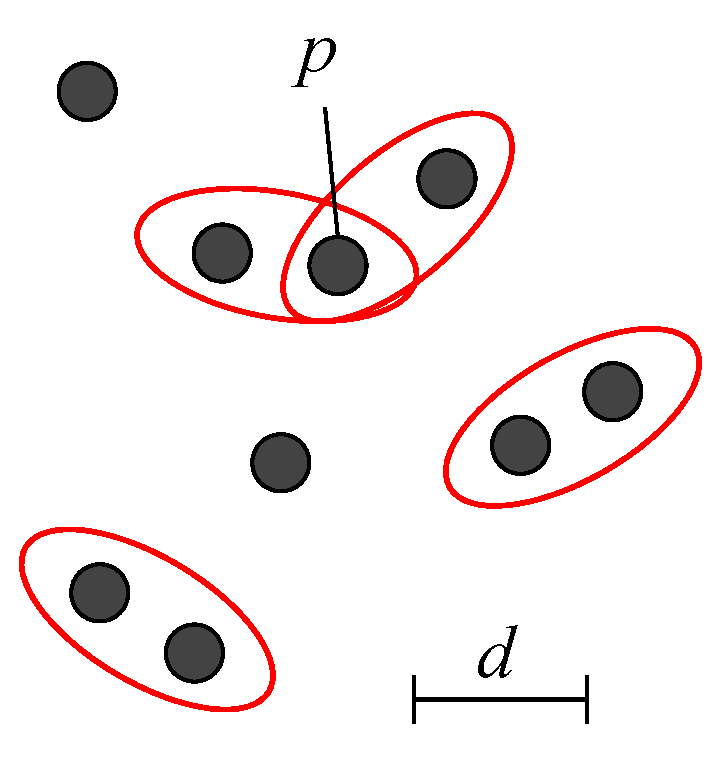
\includegraphics[scale=.3]{figs/cvl_proximity_conflicts.pdf}
\caption{Conflicts generated by the proximity constraint for distance $d$. Notice that point $p$ is a member of more than one conflict set.}
\label{fig:proximity:conflict}
\end{center}
\end{figure}

Consider a conflict set containing $k_1$ records, where at most $k_2$ of these records can be selected (where $k_1 > k_2$). Then it is equivalent to state that at least $\lambda = k_1 - k_2$ of these records must be \emph{deleted}. In the mathematical formulation of the problem in Section~\ref{sec:optimizationmodel} we will use this alternative way to formulate conflict sets.

\subsection{\hl{Selection as a combinatorial optimization problem}}
\label{sec:filtering}
Constraints must be complemented by an effective method for finding a good solution in the feasible solution space. Because of the nature of selection, records can have only two states; deleted and not deleted. This makes combinatorial optimization particularly appropriate.

The optimization problem is to select a subset of the dataset, such that all conflicts are resolved, and such that the aggregate weight of records that are not selected is minimized. In Section~\ref{sec:optimizationmodel} we present a mathematical formulation of this optimization problem.

\subsection{\hl{Selection for multiple scales}}
\label{sec:multi:scale:selection}
Besides finding a solution to the selection problem for a single scale, we are also interested in finding a series of solutions to the selection problem for a discrete set of scales or \emph{zoom levels}, i.e. solving a \emph{multi-scale selection problem}. This allows us to generalize a dataset for use in zoomable maps with discrete zoom levels.

To compute a solution to the multi-scale selection problem we use the so-called \emph{ladder} approach to multi-scale generalization~\cite{foerster2010challenges}. In this approach, the result of selecting records for a larger scale is used as input for selection at the next smaller scale. We use this approach because it has two advantages.

Firstly, by using the ladder approach, a constraint known as the \emph{zoom-consistency} constraint~\cite{sarma2012fusiontables} is automatically enforced. This constraint states that when zooming in on a map, records may only appear -- never disappear. This is arguably appropriate for most datasets. 

Secondly, the conflict sets get restricted after computing selection for the largest scale. For the proximity constraint applied to point datasets, each point can be in at most six different conflict sets. For the density constraint in the typical situation where a cell on zoom level $i$ covers an area corresponding to four cells on zoom level $i+1$, a conflict set will contain at most $4K$ records. This is easy to see.

In the case that enforcing zoom-consistency is inappropriate, e.g. when selecting regional labels were records both appear and disappear when zooming in, it would be better to use the \emph{star} approach~\cite{foerster2010challenges}. We have not implemented support for the star approach, but this is a low hanging fruit for future work.



